\documentclass[11pt]{article}

\usepackage[margin=1in]{geometry}
\usepackage{amsmath,amssymb,amsthm}
\usepackage{minted}
\newcommand{\mnt}[1]{{\small\mintinline{java}{#1}}}
\usepackage{tikz}
\usetikzlibrary{arrows}
\usepackage{hyperref}

\theoremstyle{definition}
\newtheorem{thm}{Thm}{}{}
\newtheorem{myDefinition}[thm]{Definition}{\bfseries}{}
\newtheorem{myExample}[thm]{Example}{\bfseries}{}
\newtheorem{myLemma}[thm]{Lemma}{\bfseries}{}
\newtheorem{myTheorem}[thm]{Theorem}{\bfseries}{}

\newcommand{\red}[1]{\textbf{\color{red} #1}}
\newcommand{\N}{\mathbb{N}}
\newcommand{\R}{\mathbb{R}}
\newcommand{\kstar}{^{\textstyle *}}
\newcommand{\sinf}{^\infty}
\newcommand{\serial}{\gg}
\newcommand{\sloop}{\mathsf{loop}}

\newcommand{\sensorId}{\mathit{sensorId}}
\newcommand{\val}{\mathit{val}}
\newcommand{\ts}{\mathit{ts}}
\newcommand{\avg}{\mathit{avg}}
\newcommand{\wndStartTs}{\mathit{wndStartTs}}
\newcommand{\wndEndTs}{\mathit{wndEndTs}}

\begin{document}

\title{COMP 418/518: Homework 4 \\[1ex] \large [Weight of homework: 25\% of the final grade]}
\author{Authors: Yicheng Jin yj67@rice.edu}
\date{Due on April 6, 2026 \\ \small (released on March 23, 2026)}

\maketitle

\paragraph{Instructions:}

For this homework, you should work in groups of 3--4 people (i.e., the groups that have been declared and accepted).
%
Only one member of the group should submit on Gradescope.
%
All group members must be included in the submission on the Gradescope system (otherwise no credit will be given).
%
Also specify in your submission file all the members of your group (name and NetID) using the \texttt{\textbackslash authors} macro.
%
The submission must be typed in LaTeX using the provided template.
%
The use of AI systems (including, but not limited to, ChatGPT, Gemini, Copilot, and Claude) is entirely prohibited.
%
No discussion or collaboration is allowed outside of the group.
%
Late submissions are not accepted.

\begin{center}
	You should provide \emph{pseudocode} for all the algorithms that you describe.
\end{center}

\paragraph{Grading:}

We will give a 5\% grade bonus to students taking COMP 418. The homework will be graded based on correctness, completeness, and the quality of the provided solutions.

\paragraph{Note:}

Please go over the provided Java source code, because it contains some definitions that are relevant for several questions of the homework. Unless specified otherwise, all the denotations that we consider in the problems are cumulative (i.e., they give the overall output history).

\clearpage % DO NOT REMOVE THIS
\section{The Dataflow Model [110 points]}

We will explore the dataflow model of computation. We consider dataflow graphs where each process (sometimes referred to as node, operator, actor) can be implemented using the following Java interface:
\begin{minted}{java}
public interface Operator<A,B> {
	void start(Sink<B> sink);
	void next(A item, Sink<B> sink);
}

public interface Sink<A> {
	void next(A item);
}
\end{minted}
See the uploaded code for a similar programming model.

We assume that every execution of \mnt{start} and \mnt{next} terminates and thus results in the generation of a \emph{finite} number of output items. Under this assumption, every operator can be described by a \emph{monotone} function $f: A\kstar \to B\kstar$ (cumulative denotation), where $A\kstar$ is the set of all finite words (strings) over $A$. See several lectures that discuss this concept of describing operators (streaming algorithms) using functions.

\subsection{Semantic Characterization of Statelessness [10 points]}

You are asked to give a semantic characterization of the \emph{stateless} operators, that is, those operators that can be implemented without maintaining any state across steps (examples of such operators: \mnt{id}, \mnt{filter}, and \mnt{map}). The operators \mnt{fold} and \mnt{scan}, on the other hand, are stateful. More specifically, you want to characterize the class of (computable) monotone functions $f: A\kstar \to B\kstar$ that admit a stateless implementation. Formulate precisely a property $P(f)$ so that Theorem~\ref{thm:stateless} below holds.

\paragraph{Definition of property $P(f)$:}
%
$P(f)$: There exists a function $h: A \to B\kstar$ such that for every $s \in A\kstar$ and every $a \in A$:
\[
	f(s \cdot a) = f(s) \cdot h(a).
\]
Equivalently, the \emph{incremental output} produced upon receiving input $a$ depends only on $a$ and not on the history $s$.

\begin{myTheorem}
	\label{thm:stateless}
	Let $f: A\kstar \to B\kstar$ be a computable monotone function. The function $f$ is the cumulative denotation of a stateless operator if and only if $P(f)$.
\end{myTheorem}
\begin{proof}
	$(\Rightarrow)$ Suppose $f$ is the cumulative denotation of a stateless operator. Then \mnt{start(sink)} produces some fixed output $w_0 = f(\varepsilon) \in B\kstar$, and \mnt{next(a, sink)} produces output that depends only on $a$ (no state across steps), say $h(a) \in B\kstar$. For any input $s = a_1 a_2 \cdots a_n$:
	\[
		f(a_1 \cdots a_n) = w_0 \cdot h(a_1) \cdot h(a_2) \cdots h(a_n).
	\]
	In particular, $f(s \cdot a) = f(s) \cdot h(a)$ for all $s \in A\kstar$ and $a \in A$. So $P(f)$ holds.

	$(\Leftarrow)$ Suppose $P(f)$ holds with witness function $h: A \to B\kstar$. We construct a stateless operator:
	\begin{itemize}
		\item \mnt{start(sink)}: emit the symbols of $f(\varepsilon)$ to \mnt{sink}.
		\item \mnt{next(a, sink)}: emit the symbols of $h(a)$ to \mnt{sink}. No state is needed because $h(a)$ depends only on $a$.
	\end{itemize}
	This operator uses no mutable state across calls to \mnt{next}. Its cumulative denotation on input $a_1 \cdots a_n$ is $f(\varepsilon) \cdot h(a_1) \cdots h(a_n)$, which equals $f(a_1 \cdots a_n)$ by induction using $f(s \cdot a) = f(s) \cdot h(a)$. Since $h$ is computable (it can be extracted from $f$, which is computable), the implementation is valid.
\end{proof}

\clearpage % DO NOT REMOVE THIS
\subsection{Translations Between Programming Models [25 points]}

We have used extensively a notation to describe dataflow processes using \mnt{read(channel)} to read from an input channel and \mnt{emit(channel)} to write to an output channel. This programming model was introduced by Kahn in \cite{Kahn1974KPN} and was further elaborated in \cite{KahnMacQ1977}. If you want to learn more about these seminal works you can read the survey \cite{MacQueen2009Kahn} and the notes \cite{Lee2011MoCs} (see reading list on Canvas). Consider the following Kahn process:
\begin{center}
	\begin{tikzpicture}[->, >=to, auto, node distance=1.5cm, semithick, transform shape]
		%
		\footnotesize
		%
		\node (L1) {};
		\node (L2) [below of=L1] {};
		\node (L3) [below of=L2] {};
		\node (M2) [draw, right of=L2, node distance=6cm] {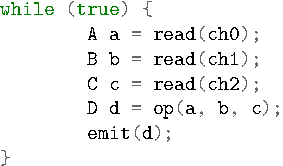
\includegraphics[scale=1.0]{zip3Kahn/zip3Kahn.pdf}};
		\node (R2) [right of=M2, node distance=5cm] {};
		%
		\path (L1) edge[bend left=15] node {\mnt{ch0: A}} (M2);
		\path (L2) edge node {\mnt{ch1: B}} (M2);
		\path (L3) edge[bend right=15] node[swap] {\mnt{ch2: C}} (M2);
		\path (M2) edge node {\mnt{ch: D}} (R2);
		%
	\end{tikzpicture}
\end{center}
Describe the same computation by implementing the \mnt{Zip3} operator of type \mnt{Operator<Or3<A,B,C>,D>}. The three input channels of the Kahn process are encoded using the disjoint union (coproduct) \mnt{Or3<A,B,C>}, which is a straightforward extension of \mnt{Or<A,B>} (see the uploaded code). Fill pseudocode in Figure~\ref{fig:zip3}. You do not have to write actual Java code for this.

\begin{figure}[t!]
	\footnotesize
	\begin{minted}[frame=single]{java}
public class Zip3<A, B, C, D> implements Operator<Or3<A,B,C>, D> {

	private final Func3<A,B,C,D> op;
	private Queue<A> bufA;
	private Queue<B> bufB;
	private Queue<C> bufC;

	public Zip3(Func3<A,B,C,D> op) {
		this.op = op;
		this.bufA = new Queue<>();
		this.bufB = new Queue<>();
		this.bufC = new Queue<>();
	}

	@Override
	public void start(Sink<D> sink) {
		// do nothing
	}

	@Override
	public void next(Or3<A,B,C> item, Sink<D> sink) {
		// item.match(
		// 	a -> bufA.enqueue(a),
		// 	b -> bufB.enqueue(b),
		// 	c -> bufC.enqueue(c)
		// );

		item.map(
			a -> bufA.enqueue(a),
			b -> bufB.enqueue(b),
			c -> bufC.enqueue(c),
		);
		
		while (!bufA.isEmpty() && !bufB.isEmpty() && !bufC.isEmpty()) {
			A a = bufA.dequeue();
			B b = bufB.dequeue();
			C c = bufC.dequeue();
			sink.next(op.apply(a, b, c));
		}
	}
}
\end{minted}
	\caption{The \mnt{Zip3} operator.}
	\label{fig:zip3}
\end{figure}

\begin{figure}[t!]
	\footnotesize
	\begin{minted}[frame=single]{java}
public class Count2 implements Operator<Or<A,A>, Nat> {

	private long count = 0;

	@Override
	public void start(Sink<Nat> sink) { /* do nothing */  }

	@Override
	public void next(Or<A,A> item, Sink<Nat> sink) {
		A a = item.map(x -> x, x -> x);
		count += 1;
		sink.next(count);
	}
}
\end{minted}
	\caption{The \mnt{Count2} operator.}
	\label{fig:count2}
\end{figure}

Consider now the operator \mnt{Count2} of type \mnt{Operator<Or<A,A>,Nat>} that is shown in Figure~\ref{fig:count2}. The input can be thought of as the interleaving of two input channels. Translate \mnt{Count2} into a Kahn process with two input channels (if possible), or prove that it is not possible to do so.

\paragraph{Operator to Kahn process translation:}

It is \textbf{not possible} to translate \mnt{Count2} into a Kahn process with two input channels.

\begin{proof}
	A Kahn process is \emph{deterministic}: at each step, it must commit to reading from a specific channel. Its input/output behavior (as a function of the two input streams) is completely determined by the contents of the two channels, regardless of the timing or interleaving of arrivals.

	Consider two scenarios with the same pair of input streams $s = (a_1)$ on \mnt{ch0} and $t = (a_2)$ on \mnt{ch1}. A Kahn process must choose which channel to read first. Suppose it reads \mnt{ch0} first:
	\begin{itemize}
		\item It reads $a_1$ from \mnt{ch0}, emits $1$, then reads $a_2$ from \mnt{ch1}, emits $2$. So the output is $(1, 2)$.
	\end{itemize}
	Now consider $s = \varepsilon$ (empty) on \mnt{ch0} and $t = (a_2)$ on \mnt{ch1}. The Kahn process tries to read \mnt{ch0} first, but \mnt{ch0} is empty, so it \emph{blocks forever}. It never reads from \mnt{ch1} and produces no output ($\varepsilon$). But \mnt{Count2} should output $(1)$ since one total item was received. Contradiction.

	A symmetric argument applies if the process reads \mnt{ch1} first. More generally, any deterministic reading schedule will block when the channel it tries to read next has no data, even though the other channel may have items. \mnt{Count2} requires a \emph{fair merge} (reacting to whichever channel has data), which is inherently \emph{non-deterministic} and cannot be expressed as a Kahn process.
\end{proof}

\clearpage % DO NOT REMOVE THIS
\subsection{Denotations [10 points]}

Describe the denotation of \mnt{Zip3} as a function $f: A\kstar \times B\kstar \times C\kstar \to D\kstar$ and the denotation of \mnt{Count2} as a function $g: A\kstar \times A\kstar \to \N\kstar$, where $\N$ is the set of the natural numbers (nonnegative integers).

\paragraph{Solution:}

\textbf{Denotation of Zip3.} Let $s = a_1 \cdots a_p \in A\kstar$, $t = b_1 \cdots b_q \in B\kstar$, $u = c_1 \cdots c_r \in C\kstar$, and let $n = \min(p, q, r)$. Then:
\[
	f(s, t, u) = \mathit{op}(a_1, b_1, c_1) \cdot \mathit{op}(a_2, b_2, c_2) \cdots \mathit{op}(a_n, b_n, c_n).
\]
That is, $f$ zips the three streams element-wise and applies $\mathit{op}$, producing output only up to the length of the shortest input stream.

\textbf{Denotation of Count2.} Let $s \in A\kstar$ and $t \in A\kstar$ with $|s| = p$ and $|t| = q$. Then:
\[
	g(s, t) = 1 \cdot 2 \cdots (p + q).
\]
That is, $g(s, t)$ is the sequence $(1, 2, \ldots, p + q)$. The output is simply the running count of the total number of items received from both channels, regardless of the interleaving order or the values of the items.

\clearpage % DO NOT REMOVE THIS
\subsection{Data Parallelism [25 points]}

In applications that require the processing of massive amounts of data (e.g., data generated by a large number of high-resolution sensors) it is often desirable to exploit \emph{data parallelism}. This is what the distributed data processing systems MapReduce, Spark, Storm and others do. As a simple example of this, consider a pipeline consisting of two \mnt{map} operators:
\begin{center}
	\begin{tikzpicture}[->, >=to, auto, node distance=3cm, semithick, transform shape]
		%
		\footnotesize
		%
		\node (M1) {};
		\node (M2) [draw, right of=M1] {\mnt{map(f)}};
		\node (M3) [draw, right of=M2] {\mnt{map(g)}};
		\node (M4) [right of=M3] {};
		%
		\path (M1) edge node {\mnt{A}} (M2);
		\path (M2) edge node {\mnt{B}} (M3);
		\path (M3) edge node {\mnt{C}} (M4);
	\end{tikzpicture}
\end{center}
We wish to parallelize this pipeline by creating several instances of \mnt{map(f)} and \mnt{map(g)} that compute independently. This is a meaningful transformation when \mnt{f} and \mnt{g} are computationally expensive. This transformation gives rise to dataflow graph of Figure~\ref{fig:data_parallelism}.

\begin{figure}[t]
	\centering
	\begin{tikzpicture}[->, >=to, auto, node distance=1.5cm, semithick, transform shape]
		%
		\footnotesize
		%
		\node (M1) {};
		\node (M2) [draw, right of=M1, node distance=2cm] {\mnt{split}};
		\node (M3) [draw, right of=M2, node distance=3cm] {\mnt{map(f)}};
		\node (M4) [draw, right of=M3, node distance=4cm] {\mnt{map(g)}};
		\node (M5) [draw, right of=M4, node distance=3cm] {\mnt{merge}};
		\node (M6) [right of=M5, node distance=2cm] {};
		%
		\node (T3) [draw, above of=M3] {\mnt{map(f)}};
		\node (T4) [draw, above of=M4] {\mnt{map(g)}};
		%
		\node (B3) [draw, below of=M3] {\mnt{map(f)}};
		\node (B4) [draw, below of=M4] {\mnt{map(g)}};
		%
		\path (M1) edge node {\mnt{A}} (M2);
		\path (M2) edge[bend left] node {\mnt{A}} (T3);
		\path (M2) edge node {\mnt{A}} (M3);
		\path (M2) edge[bend right] node[swap] {\mnt{A}} (B3);
		\path (T3) edge node {\mnt{B}} (T4);
		\path (T3) edge (M4);
		\path (T3) edge (B4);
		\path (M3) edge (T4);
		\path (M3) edge (M4);
		\path (M3) edge (B4);
		\path (B3) edge (T4);
		\path (B3) edge (M4);
		\path (B3) edge node[swap] {\mnt{B}} (B4);
		\path (T4) edge[bend left] node {\mnt{C}} (M5);
		\path (M4) edge node {\mnt{C}} (M5);
		\path (B4) edge[bend right] node[swap] {\mnt{C}} (M5);
		\path (M5) edge node {\mnt{C}} (M6);
	\end{tikzpicture}
	\caption{Extracting data parallelism from a simple pipeline of stateless operators.}
	\label{fig:data_parallelism}
\end{figure}

Describe each of the nodes (processes) of the dataflow graph of Figure~\ref{fig:data_parallelism}. You can assume that every communication channel is reliable (no messages are lost) and behaves like a FIFO buffer. Make sure that the behavior of the graph of Figure~\ref{fig:data_parallelism} (in terms of the input/output function) is exactly the same as the behavior of the original pipeline. Does this require making any noteworthy changes to the graph? You may have to introduce new notation for writing pseudocode that describes the nodes. Try to make your notation intuitive and explain the aspects that are not obvious. You do not have to restrict yourself to Kahn processes for the code that runs on each node.

\paragraph{Solution:}

We use the notation \mnt{read(ch)} for blocking read from a channel and \mnt{emit(ch, v)} for writing value $v$ to a channel. We denote the three parallel lanes as lane $0$, $1$, $2$. Each item is tagged with a \emph{sequence number} to allow the merge node to reconstruct the original order.

\paragraph{Noteworthy change to the graph:} The diagram shows a \emph{fully connected} bipartite graph between the \mnt{map(f)} and \mnt{map(g)} stages (9 edges). However, for correctness we only need each \mnt{map(f)}$_k$ to send to the corresponding \mnt{map(g)}$_k$ on the same lane (3 edges). The cross-lane connections are unnecessary and would cause incorrect duplicate processing. So the graph should be simplified to have only the 3 direct lane connections between the two stages.

\paragraph{Split node:}
\begin{minted}[frame=single]{java}
// Distributes items round-robin across 3 lanes, tagging with sequence number
seq = 0;
while (true) {
    A a = read(input);
    lane = seq % 3;
    emit(out[lane], (a, seq));   // send tagged item to lane
    seq++;
}
\end{minted}

\paragraph{Map(f)$_k$ node} (for lane $k \in \{0, 1, 2\}$):
\begin{minted}[frame=single]{java}
// Applies f to each item, passes along the sequence number
while (true) {
    (A a, int seq) = read(in_k);
    B b = f(a);
    emit(out_k, (b, seq));
}
\end{minted}

\paragraph{Map(g)$_k$ node} (for lane $k \in \{0, 1, 2\}$):
\begin{minted}[frame=single]{java}
// Applies g to each item, passes along the sequence number
while (true) {
    (B b, int seq) = read(in_k);
    C c = g(b);
    emit(out_k, (c, seq));
}
\end{minted}

% need to be fixed (can use fangzhou's code here)

\paragraph{Merge node:}
Fangzhou here !
% \begin{minted}[frame=single]{java}
% // Reassembles output in original sequence order
% nextSeq = 0;
% buffer = new HashMap<Int, C>();   // seq -> value
% while (true) {
%     // Read from the lane that has the next expected item
%     lane = nextSeq % 3;
%     (C c, int seq) = read(in[lane]);
%     // Since round-robin split guarantees in-order arrival per lane,
%     // seq == nextSeq is always true here
%     emit(output, c);
%     nextSeq++;
% }
% \end{minted}

\paragraph{Correctness argument:} Since \mnt{split} distributes items in round-robin order (item $i$ goes to lane $i \bmod 3$), the \mnt{merge} node knows exactly which lane holds the next item in sequence. It reads from lane $\mathit{nextSeq} \bmod 3$, which is deterministic and requires no buffering. The overall input/output function is: for input $a_1 a_2 \cdots a_n$, the output is $g(f(a_1)) \cdot g(f(a_2)) \cdots g(f(a_n))$, which is identical to the original pipeline \mnt{map(f)} $\serial$ \mnt{map(g)}.

\clearpage % DO NOT REMOVE THIS
\subsection{Disorder and Watermarks [40 points]}

Consider an IoT application that requires collecting data from a large and physically distributed collection of smart sensors. All sensor streams are sent to a centralized location (``server'') for processing. Because of the physical distribution, the data can arrive disordered. The server sees a single input stream of data items of the form $(\sensorId, \val, \ts): \N \times \R \times \N$, where $\sensorId: \N$ is a unique identifier for a sensor, $\val: \R$ is the sensor measurement, and $\ts: \N$ is a timestamp that measures time in msec (milliseconds). The data items in the input stream may be \emph{disordered} with respect to the timestamp. So, we \emph{cannot} expect in general that the data will appear in non-decreasing timestamp order.

We define the \emph{watermark} of the input stream to be the maximum timestamp seen so far\footnote{Similar notions of watermarks are considered in many data stream processing systems. For example, see \url{https://learn.microsoft.com/en-us/azure/stream-analytics/stream-analytics-time-handling} and \url{https://www.databricks.com/blog/feature-deep-dive-watermarking-apache-spark-structured-streaming}.}. We make a \emph{bounded lateness} assumption, namely that each data item should be at most $T \geq 0$ time units behind the watermark. That is, if $(\sensorId, \val, \ts)$ is the current data item and $t$ is the current watermark, then it should hold that $t - \ts \leq T$.

We want to compute the \emph{tumbling window average} of the measurement values. Suppose that $W > 0$ is the length of the window. For each time interval $[0, W), [W, 2W), [2W, 3W), \ldots$ we want to output the average value of all measurements that belong to the interval according to their timestamp. The output should be of the form $(\avg, \wndStartTs, \wndEndTs): \R \times \N \times \N$, where $\avg: \R$ is the average measurement of the window, $\N$ is the start time of the window, and $\N$ is the end time of the window. E.g., if $y_0$ is the average of the window $[0, W)$, then the output should be $(y_0, 0, W - 1)$.
\begin{center}
	\begin{tikzpicture}[->, >=to, auto, node distance=6cm, semithick, transform shape]
		%
		\footnotesize
		%
		\node (M1) {};
		\node (M2) [draw, right of=M1] {\mnt{tumbling-window(W, val, average)}};
		\node (M3) [right of=M2] {};
		%
		\path (M1) edge node {$\N \times \R \times \N$} (M2);
		\path (M2) edge node {$\R \times \N \times \N$} (M3);
	\end{tikzpicture}
\end{center}
You should emit the output for a window as early as possible, i.e., as soon as it becomes apparent that no other measurement of the window will be seen in the future (recall the bounded lateness assumption).

Provide detailed streaming pseudocode for the most efficient implementation of this tumbling window operator that you can think of. Discuss the memory and time-per-item complexity of your implementation.

\paragraph{Solution:}

\paragraph{Key idea.} We maintain per-window aggregates (sum and count). The watermark is the maximum timestamp seen so far. A window $[kW, (k{+}1)W)$ is emitted as soon as the watermark guarantees no future item can belong to it: this happens when $\mathit{watermark} \geq (k{+}1)W + T$, because the bounded lateness assumption ensures every future item has $\ts \geq \mathit{watermark} - T \geq (k{+}1)W$, which falls outside window $k$.

\paragraph{Pseudocode:}
\begin{minted}[frame=single]{java}
// State
watermark = 0;
windows = new HashMap<Int, (Double sum, Int count)>();
nextWindowToEmit = 0;  // index of the earliest un-emitted window

// Operator interface
void start(Sink<(Real, Nat, Nat)> sink) {
    // do nothing
}

void next((Nat sensorId, Real val, Nat ts), Sink<(Real, Nat, Nat)> sink) {
    // 1. Update watermark
    watermark = max(watermark, ts);

    // 2. Assign item to its window and update aggregate
    int k = ts / W;   // integer division: window index
    if (windows.containsKey(k)) {
        windows[k].sum += val;
        windows[k].count += 1;
    } else {
        windows[k] = (val, 1);
    }


	// need to be fixed, store old watermark, the complexity of per item may not be O(1), 如果T, W是 constants 是O(1), variable 是O(T/W)

    // 3. Emit all windows that are now complete
    //    Window k is complete when watermark >= (k+1)*W + T
    while (nextWindowToEmit * W + W + T <= watermark) {
        int k = nextWindowToEmit;
        if (windows.containsKey(k)) {
            Real avg = windows[k].sum / windows[k].count;
            sink.next((avg, k * W, (k+1) * W - 1));
            windows.remove(k);
        }
        // If no items fell in this window, skip it (no output)
        nextWindowToEmit++;
    }
}
\end{minted}

\paragraph{Complexity analysis.}

\begin{itemize}
	\item \textbf{Time per item:} Updating the watermark and inserting into the window map are both $O(1)$ (using a hash map). The \mnt{while} loop emits completed windows. Each window is emitted at most once across the entire stream, so the total cost of all emissions is proportional to the number of windows emitted. Amortized over all items, the cost per item is $O(1)$.

	\item \textbf{Memory:} At any point, the active (un-emitted) windows are those with index $k \geq \mathit{nextWindowToEmit}$ that have received at least one item. Since all items satisfy $\ts \geq \mathit{watermark} - T$, the timestamps of buffered items span a range of at most $T + W$. Therefore, the number of active windows is at most $\lfloor T/W \rfloor + 2$. Each window stores a sum and a count, so the total memory is $O(T/W + 1)$.
\end{itemize}

\clearpage % DO NOT REMOVE THIS
\section{Denotational Semantics of Kahn Process Networks [40 points]}

\begin{myLemma}
	Let $A$ and $B$ be $\omega$-CPOs. Then, $A \times B$ is an $\omega$-CPO.
\end{myLemma}
\begin{proof}
	\red{Fill me in.}
\end{proof}

\begin{myLemma}
	Let $A$, $B$ and $C$ be $\omega$-CPOs. Suppose that $f: A \to B$ and $g: B \to C$ are $\omega$-continuous. Then, the serial composition $f \serial g: A \to C$ is $\omega$-continuous. Recall from the lectures that $(f \serial g)(a) = g(f(a))$ for every $a \in A$.
\end{myLemma}
\begin{proof}
	\red{Fill me in.}
\end{proof}

We will consider now the \textbf{\em semantics of feedback} using an interesting example. Consider the Kahn process shown below:
\begin{center}
	\begin{tikzpicture}[->, >=to, auto, node distance=1.5cm, semithick, transform shape]
		%
		\footnotesize
		%
		\node (L1) {};
		\node (L2) [below of=L1] {};
		\node (L3) [below of=L2] {};
		\node (M2) [draw, right of=L2, node distance=6cm] {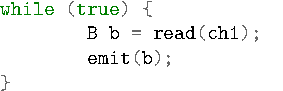
\includegraphics[scale=1.0]{projKahn/projKahn.pdf}};
		\node (R2) [right of=M2, node distance=5cm] {};
		%
		\path (L1) edge[bend left=10] node {\mnt{ch0: A}} (M2);
		\path (L3) edge[bend right=10] node[swap] {\mnt{ch1: B}} (M2);
		\path (M2) edge node {\mnt{ch: B}} (R2);
		%
	\end{tikzpicture}
\end{center}
The (cumulative) input/output behavior of this process can be described by an $\omega$-continuous function $f: A\sinf \times B\sinf \to B\sinf$. Describe the function $f$ and the function $\sloop(f): A\sinf \to B\sinf$ ($\sloop$ is feedback composition, as defined in the lectures).

\paragraph{Solution:}

\red{Fill me in.}

\clearpage % DO NOT REMOVE THIS
\section{ToyDSL [100 points]}

Download the Java project form Canvas. Carefully read all the provided code in order to understand the programming model that we consider. Implement the ToyDSL domain-specific language using the included instructions. Your implementation should pass all included unit tests. If there is anything that you would like to clarify, please do so below.

\subsection*{Solution}

\red{Fill me in.}


\bibliographystyle{plain}
\bibliography{refs}

\end{document}